\documentclass[
  digital,
  oneside,
  nosansbold,
  nocolorbold,
  lof,
  lot
]{fithesis4}

\usepackage[resetfonts]{cmap}
\usepackage[T1]{fontenc}
\usepackage[
  main=english,
  english, german, czech, slovak
]{babel}

\usepackage{paratype}

\thesissetup{
    date        = \the\year/\the\month/\the\day,
    university  = mu,
    faculty     = fi,
    type        = bc,
    department  = Department of Computer Science,
    author      = Petr Kubica,
    gender      = m,
    advisor     = {RNDr. Jan Mrázek.},
    title       = {Jaculus: Approachable Programming of Embedded Devices via Javascript},
    TeXtitle    = {Jaculus: Approachable Programming of Embedded Devices via Javascript},
    keywords    = {keyword1, keyword2, ...},
    TeXkeywords = {keyword1, keyword2, \ldots},
    abstract    = {
      This is the abstract of my thesis, which can

      span multiple paragraphs.
    },
    thanks      = {
      These are the acknowledgements for my thesis, which can

      span multiple paragraphs.
    },
    bib         = bibliography.bib,
    facultyLogo = fithesis-fi,
}
\usepackage{makeidx}
\makeindex
\usepackage{paralist}
\usepackage{url}
\usepackage{markdown}
\def\markdownRendererCodeSpan#1{\colorbox{gray!10}{#1}}
\usepackage{listings}
\lstset{
  basicstyle       = \small\ttfamily,
  identifierstyle  = \color{black},
  keywordstyle     = \color{blue},
  keywordstyle     = {[2]\color{cyan}},
  keywordstyle     = {[3]\color{olive}},
  stringstyle      = \color{red},
  commentstyle     = \itshape\color{teal},
  breaklines       = true,
  showstringspaces = false,
  backgroundcolor  = \color{gray!10},
}
\usepackage{floatrow}
\floatsetup[table]{capposition=top}
\usepackage[babel]{csquotes}


\lstdefinelanguage{js}{
  keywords={typeof, new, true, false, catch, function, return, null, catch, switch, var, if, in, while, do, else, case, break},
  ndkeywords={class, export, boolean, throw, implements, import, this},
  comment=[l]{//},
  morecomment=[s]{/*}{*/},
  morestring=[b]',
  morestring=[b]",
}

\lstdefinelanguage{cpp}{
  keywords={alignas, alignof, and, and_eq, asm, atomic_cancel, atomic_commit, atomic_noexcept, auto, bitand, bitor, bool, break, case, catch, char, char8_t, char16_t, char32_t, class, compl, concept, const, consteval, constexpr, constinit, const_cast, continue, co_await, co_return, co_yield, decltype, default, delete, do, double, dynamic_cast, else, enum, explicit, export, extern, false, float, for, friend, goto, if, inline, int, long, mutable, namespace, new, noexcept, not, not_eq, nullptr, operator, or, or_eq, private, protected, public, reflexpr, register, reinterpret_cast, requires, return, short, signed, sizeof, static, static_assert, static_cast, struct, switch, synchronized, template, this, thread_local, throw, true, try, typedef, typeid, typename, union, unsigned, using, virtual, void, volatile, wchar_t, while, xor, xor_eq},
  comment=[l]{//},
  morecomment=[s]{/*}{*/},
  morecomment=[l][\color{violet}]{\#},
  morestring=[b]',
  morestring=[b]",
}


\begin{document}
\shorthandoff{'}
\begin{markdown*}{%
  hybrid,
  definitionLists,
  footnotes,
  inlineFootnotes,
  hashEnumerators,
  fencedCode,
  citations,
  citationNbsps,
  pipeTables,
  tableCaptions,
}

\chapter{Motivation}

Microcontrollers in embedded devices are typically programmed in compiled languages, such as C, C++, or Rust. Although these languages provide high performance and low overhead at runtime, they can be difficult to learn and use. Another problem of compiled languages in embedded environments is often a long build and deployment time, as the final executable usually contains the full firmware, including all built-in libraries. This, in turn, causes a long development cycle and idle time for the developer.

Most embedded applications have reactive and asynchronous elements, which are difficult to express in low-level languages. This induces a lot of boilerplate code, which obfuscates the main application logic and makes it harder to develop and maintain. Even though high-level languages such as C++ and Rust somewhat alleviate this problem, C is often the only language with direct support from the manufacturers, which again adds more work for the developer.

\chapter{Proposed solution}

The proposed solution is to use a high-level, interpreted language instead.

JavaScript was chosen for its popularity and low hardware requirements of some of its implementations. It also maps very well to the event-centered nature of many embedded systems, as JavaScript is inherently event-driven.

Because JavaScript is weakly typed, debugging errors caused by type mismatches is sometimes challenging. A possible solution is to use a strongly typed language, such as TypeScript. However, as compiling or running TypeScript on a microcontroller is not feasible, it must first be compiled to JavaScript.

\chapter{Approach}

A JavaScript engine is needed to interpret JavaScript code. The chosen engine is QuickJS, a small, embeddable C implementation of the ECMAScript 2020 specification. Compared to other popular options -- DukTape, MujJS, and XS -- it stands on a nice middle ground regarding the feature set, performance, and memory footprint.

The whole solution is split into multiple components:

  - Jaculus-machine -- standalone, embeddable, C++ centric JavaScript runtime using QuickJS at its core
  - Jaculus-link -- standalone communication library for multiplexing multiple channels on a single stream connection
  - Jaculus-device-core -- core library for creating new Jaculus devices
  - Jaculus-tools -- a command-line application for controlling and monitoring Jaculus devices
  - Jaculus-esp32 -- Jaculus device port for the ESP32 platform (with verified support for ESP32 and ESP32-S3 WROOM modules)

This approach allows for the creation of Jaculus devices, which give complete control over the device to the JavaScript runtime, or applications whose main logic is written in C++ and which only embed the JavaScript runtime as a part of the application. The use case for the latter are, for example, devices used as game elements, where the low-level logic (e.g., communication, user interface) is written in C++, and the highly abstracted game logic is written in JavaScript.


\chapter{Overview}

\subsection{JavaScript}

JavaScript is a high-level, interpreted, weakly and dynamically typed programming language. It is standardized in the ECMAScript specification, which is maintained by Ecma International.

Although JavaScript programs are event-driven, the code is executed in a single thread. This is achieved by using an event loop, where asynchronous events are queued and executed in the order they are received. Therefore, JavaScript programs must be written in a non-blocking manner, as blocking the event loop will cause the program to stop responding to events. Events are generated by the JavaScript engine or the host environment synchronously and asynchronously.


\subsection{TypeScript}

TypeScript is a strongly typed superset of JavaScript. It is developed and maintained by Microsoft. TypeScript is compiled to JavaScript and can be used in any JavaScript environment that supports the selected ECMAScript version.


\subsection{QuickJS}

QuickJS is a JavaScript engine implementing the ECMAScript 2020 specification. It was developed by Fabrice Bellard and is licensed under the MIT license. It is written in C and is designed to be embeddable in other applications.

QuickJS uses POSIX for atomic operations and system time. Although this slightly limits its portability. Fortunately, ESP-IDF, the main target platform for Jaculus, supports POSIX. For supporting other platforms, a custom implementation of the interface would have to be provided.

JavaScript program is executed in a Realm, which defines the execution environment (e.g., global object and set of built-in objects). QuickJS uses a different term for this concept -- Context, which I will be using throughout this thesis, as it is also used in the source code.


\subsection{Jaculus device}

A Jaculus device is a device that runs firmware built on top of the Jaculus-device-core library and which gives complete control over the device to the JavaScript runtime. The device can be controlled using the Jaculus-tools.


\chapter{Jaculus-machine}

Jaculus-machine is a standalone, embeddable, C++ centric JavaScript runtime based on QuickJS. The main goal of Jaculus-machine is to provide a simple and easy-to-use API for adding features to the runtime.

A large part of Jaculus-machine is a set of C++ classes that wrap the QuickJS API. The classes provide RAII semantics and an easy-to-use API for the most common use cases.

Jaculus-machine uses two core concepts, which I will refer to as *Machine* and *Feature* throughout the rest of this thesis.

  - *Machine* -- an instance of the runtime complete with all the selected *Features*
  - *Feature* -- a component that can be used as a part of a *Machine* and which provides functionality to the runtime or to other *Features*

\section{Architecture}

\subsection{Machine and Features}

*Machine* is defined using stack inheritance from `jac::MachineBase` and selected *Feature* classes. The `jac::MachineBase` class provides only the most basic functionality of the runtime, whereas the *Feature* classes provide additional functionality, such as an event loop, filesystem access, etc.

An example definition of a *Machine* type may look like this:

```cpp
using Machine =
    ModuleLoaderFeature<
    FilesystemFeature<
    StdioFeature<
    BasicStreamFeature<
    jac::MachineBase
>>>>;
```

The stack design of *Machine* allows interfacing with different *Features* in C++ directly without any middleware. Lower-level *Features* are located lower in the stack and implement platform-specific functionality, while higher-level *Features* are located higher in the stack and can use the abstraction provided by the lower-level *Features*. This allows for easy portability of higher-level *Features* to other platforms.

*Features*, which export functionality to the JavaScript environment, should also provide the same functionality to other *Features* in a way that is as close to the JavaScript API as possible. When a *Feature* defines a JavaScript module, it should wrap the module functionality in a member class instance so that other *Features* can access the functionality as `this->moduleName.function()`.

\subsection{Exceptions}

Jaculus-machine provides a set of wrappers that allow usage of C++ code in the runtime. When an exception is thrown in the C++ code, it is caught by the wrapper, converted to a JavaScript exception, and propagated to the runtime. The library allows the user to specify the type of JavaScript `Error` or any other JavaScript value that should be thrown.

Similarly, when a JavaScript exception is thrown in the runtime, it is caught by its wrapper, converted to a C++ exception of type `jac::Exception`, and propagated to the C++ code.


\section{Features}

Jaculus-machine adds a minimum set of features to the runtime but provides tools that make creating new *Features* as easy as possible.

\subsection{Value wrapping and conversion}

QuickJS uses reference counting for memory management, and the user is responsible for freeing JavaScript values when they are no longer needed. Jaculus-machine provides a set of classes that wrap JavaScript values and provide RAII semantics for them. The classes also provide a simple API for converting to and from C++ types.

The base class for JavaScript value wrapper is `jac::ValueWrapper` and provides a general API for working with JavaScript values. More specific wrapper classes are derived from `jac::ValueWrapper` and provide additional functionality, such as `jac::ObjectWrapper` and `jac::FunctionWrapper`.

The wrapped value can be either a value (e.g., a number) or a reference (e.g., an object).
`jac::ValueWrapper` has a template parameter `managed` that defines whether the wrapper takes ownership of the underlying JavaScript value. This pattern is assumed from QuickJS, which sometimes does not give ownership of the value to the user to reduce the number of changes in its reference count. If the value is a reference, depending on the value of `managed`, the wrapper will either be a strong or a weak reference to the value. For convenience, the library provides two type aliases for all built-in wrappers, which are usually used instead and follow the following pattern:

```cpp
// value/strong reference
using Value = ValueWrapper<true>;
// value/weak reference
using ValueWeak = ValueWrapper<false>;
```

Default conversions for some built-in types are provided, such as `int`, `double`, `std::string`, and `std::vector`. The library also provides a mechanism for defining custom conversions for user-defined (and not-yet-supported built-in) types.

Many of these conversions are done automatically in, among others, getters, setters, and function calls. This allows for wrapping existing functions without having to write conversion code manually.

\subsection{Function wrapping}

The library provides an interface for defining JavaScript functions by wrapping almost any existing callable C++ object. This interface is presented in the form of `jac::FunctionFactory` class. Because variadic functions in C++ are processed at build time, they can not be universally wrapped. For this reason, `jac::FunctionFactory` lets the user define a function with an argument of type `std::vector<jac::ValueWrapper>`, which, when called, will contain the arguments passed to the function.

The created wrapper then automatically performs argument and return value type conversions and wraps any exceptions thrown by the wrapped function in a JavaScript exception.

\subsection{Class wrapping}

The library provides an interface for defining JavaScript classes, which can contain opaque C++ objects. The user must first define a `ProtoBuilder` class, which tells the library how to construct the JavaScript object prototype. The class `jac::Class` can then be used to initialize the class in a given Context, construct the JavaScript object or obtain its constructor.

\subsection{Built-in *Features*}

The following *Features* are included with the library (their class names are suffixed with "Feature"):

  - EventQueue -- an asynchronous event queue that can be used to schedule events to be executed in the event loop; the events can be scheduled from any thread
  - EventLoop -- an event loop that uses an event queue to execute events in the main thread
  - Filesystem -- an abstraction over the filesystem that provides access to files and directories
  - ModuleLoader -- an implementation of module loader for loading modules from the filesystem (using the `import` statement in JavaScript) and evaluating JavaScript files (using the `eval` function in C++)
  - BasicStream -- an implementation of basic readable and writable stream types
  - Stdio -- a feature that adds `stdin`, `stdout`, and `stderr` streams to the *Machine* and `console` interface only to the runtime
  - Timers -- typical JavaScript timers and a sleep function

\subsection{Watchdog}

The `jac::MachineBase` class provides a watchdog that can be used to detect infinite loops in the runtime. The watchdog can be configured using the `setWatchdogTimeout` method. By setting the timeout to 0, the watchdog can be disabled. The watchdog is disabled by default.

By default, the watchdog will interrupt the runtime on timeout. This behavior can be changed by setting the watchdog handler using the `setWatchdogHandler` method. Instead of interrupting, the handler will be called, and if it returns `true`, the watchdog will interrupt the runtime. If the handler returns `false`, the machine will continue to run, but the watchdog will not be reset.


\section{Implementation}

- ISO C++ 20, QuickJS - posix

\subsection{Default event loop}

Default event loop implementation is split into two separate *Features*. One implements an event queue, and the other implements the event loop. This allows for easier portability, as the event loop itself can be reused on different platforms, while the event queue can be extended to, for example, support scheduling events from interrupts.


\section{Usage}

\subsection{Adding the library to a project}

The library is configured as a CMake project. It exports a CMake target called `jac-machine` that can be linked to other projects.

\subsection{Creating a *Machine*}

 1. The user must define the the *Machine* type using inheritance from `jac::MachineBase` and selected *Features*, as described in ((TODO)).

 2. The *Machine* type can be used to create an instance of the *Machine*:

```cpp
Machine machine;
```

 3. The user can configure the *Machine* and its *Features* using their provided interface. The runtime is still not initialized, and the user must not interact with it.

 4. After configuration the user must initialize the *Machine*:

```cpp
machine.initialize();
```

 5. The *Machine* is now configured, initialized, and ready to use.

\subsection{Running JavaScript code}

Using the `eval` method, the *Machine* can evaluate JavaScript code from a string. The `eval` method takes the code to evaluate, the filename of the code (used for error reporting), and a set of flags that control the evaluation Context. The following code evaluates a simple "Hello, world!" program:

```cpp
// jac::MachineBase::eval(std::string code, std::string filename, jac::EvalFlags flags)
machine.eval("console.log('Hello, world!');", "<eval>", jac::EvalFlags::Global);
```

The return value of the `eval` method is a `jac::ValueWrapper`, which contains the result of the evaluation. In this case, the result is `undefined` and is ignored.

To evaluate a file, `ModuleLoaderFeature::evalFile` method can be used:

```cpp
// jac::ModuleLoaderFeature::evalFile(std::string filename)
machine.moduleLoaderFeature.evalFile("hello.js");
```

Any unhandled exceptions thrown by the evaluated code will be wrapped to C++ exceptions of type `jac::Exception` and thrown by the `eval` method.

\subsection{Running the event loop}

After evaluating some code, the execution will stop. To continue execution, the user must run the event loop, which can be done using the `EventLoopFeature::runEventLoop` method:

```cpp
machine.runEventLoop();
```

The `runEventLoop` method will block until the event loop is stopped. It must be stopped manually either by calling the `EventLoopFeature::stop`, `EventLoopFeature::kill`, or JavaScript function `exit`.

If an unhandled exception is thrown by the event loop, it will be wrapped to C++ exception of type `jac::Exception` and thrown by the `runEventLoop` method. The event loop will also be stopped.

\subsection{JavaScript values}

As described in ((TODO)), the library provides a mechanism for wrapping JavaScript values.

New JavaScript values can be created using static methods of the `jac::ValueWrapper` and its subclasses. The following code shows some examples:

```cpp
ContextRef ctx = ...;

jac::Value undefined = jac::Value::undefined(ctx);
jac::Value number = jac::Value::from<int>(ctx, 42);
jac::Value string = jac::Value::from<std::string>(ctx, "Hello, world!");
jac::Value object = jac::Object::create(ctx);
jac::Value array = jac::Array::create(ctx);
```

The `jac::ValueWrapper` class provides methods for converting the wrapped value to a C++ value:

```cpp
jac::Value value = ...;

int number = value.to<int>();
std::string string = value.to<std::string>();
```

If the wrapped value cannot be converted to the requested type, a `jac::Exception` will be thrown.

\subsection{JavaScript exceptions}

If wrapped C++ code throws an exception, it will be wrapped to a JavaScript exception and thrown to the JavaScript code. The following exception types are converted as follows:

  - `jac::Exception` -- the exception is converted to a specified `Error` type, or a specified value is thrown
  - `std::exception` -- the exception is converted to an `Error` object with the exception message
  - any other exception -- the exception is converted to an `Error` object with the message "unknown exception"

To create a `jac::Exception` that will be thrown to JavaScript as a specified `Error` type, the `jac::Exception::create` method can be used:

```cpp
ContextRef ctx = ...;

jac::Exception::create(ctx, jac::Exception::Type::TypeError, "invalid argument");
```

To create a `jac::Exception` that will be thrown to JavaScript as a specified value, the value can be converted to a `jac::Exception` using the `jac::ValueWrapper::to` method:

```cpp
ContextRef ctx = ...;

jac::Value value = ...;
jac::Exception exception = value.to<jac::Exception>();
```

\subsection{Wrapping C++ functions}

The library provides a mechanism for wrapping C++ functions to be called from JavaScript as described in ((TODO)).

C++ functions can be wrapped using the `jac::FunctionFactory` class. The following code shows some examples:

```cpp
ContextRef ctx = ...;

jac::FunctionFactory ff(ctx);

ff.newFunction([](int a, int b) { return a + b; });

ff.newFunctionVariadic([](const std::vector<int> args) {
    int sum = 0;
    for (int arg : args) {
        sum += arg;
    }
    return sum;
});
```

Sometimes, the user might want to wrap a function, which has access to `this` value. The `newFunctionThis` and `newFunctionThisVariadic` methods can be used for this purpose:

```cpp
ContextRef ctx = ...;

jac::FunctionFactory ff(ctx);

ff.newFunctionThis([](jac::Value thisValue, int a, int b) {
    return thisValue.to<int>() + a + b;
});

ff.newFunctionThisVariadic([](jac::Value thisValue, const std::vector<int> args) {
    int sum = thisValue.to<int>();
    for (int arg : args) {
        sum += arg;
    }
    return sum;
});
```

\subsection{JavaScript classes}

The library provides a mechanism for creating JavaScript classes. These classes can contain opaque C++ data, as described in ((TODO)).

  1. To create a class, the user must first define a `ProtoBuilder` struct. The `ProtoBuilder` describes the class's behavior and properties using static methods. Its features are specified by inheriting from structs from the `jac::ProtoBuilder` namespace and overriding their **static** interface. The base structs also provide some convenience functions for describing the class. The following code shows some examples:

```cpp
using namespace jac;

struct MyBuilder : public ProtoBuilder::Properties {
    static void addProperties(ContextRef ctx, Object proto) {
        proto.defineProperty("foo", Value::from(ctx, 42));
    }
};

struct MyBuilder2 : public ProtoBuilder::Callable {
    static Value callFunction(ContextRef ctx, ValueWeak funcObj, ValueWeak thisVal, std::vector<ValueWeak> args) {
        return Value::from(ctx, static_cast<int>(args.size()));
    }

    // the default implementation - does not have to be overridden if not needed
    static Value callConstructor(ContextRef ctx, ValueWeak funcObj, ValueWeak target, std::vector<ValueWeak> args) {
        throw Exception::create(ctx, Exception::Type::TypeError, "Class cannot be called as a constructor");
    }
};

struct MyBuilder3 : public ProtoBuilder::Opaque<MyClass>, public ProtoBuilder::Properties {
    static MyClass* constructOpaque(ContextRef ctx, std::vector<ValueWeak> args) {
        return new MyClass();
    }

    // the default implementation - does not have to be overridden if not needed
    static void destructOpaque(JSRuntime* rt, MyClass* ptr) {
        delete ptr;
    }

    static void addProperties(ContextRef ctx, Object proto) {
        addPropMember<int, &MyClass::foo>(ctx, proto, "foo");
    }
};
```

  2. The `jac::Class` template can be instantiated with the `ProtoBuilder` struct to create a class definition and a name can be assigned using the `init` method. The `init` method can be called repeatedly without any effect if called with the same name; otherwise, an exception will be thrown. The following code shows some examples:

```cpp
using MyClass = Class<MyBuilder>;

void foo() {
    MyClass::init("MyClass");
}
```

  3. To use the class in a given Context, the Context must be initialized with the class definition:

```cpp
ContextRef ctx = ...;

MyClass::init(ctx);
```

  4. The user can now get the class constructor and prototype and instantiate the class:

```cpp
ContextRef ctx = ...;

void bar() {
    MyClass::init(ctx);

    Value constructor = MyClass::getConstructor(ctx);
    Value prototype = MyClass::getPrototype(ctx);

    Value obj = constructor.to<Function>().callConstructor();
};
```

\subsection{Creating new Features}

To create a new Feature, the user must define a *Feature* class. The first template parameter of the call must be `Next` from which the class inherits. To add functionality to the machine, the class may:

  - present a public interface to *Features* higher in the inheritance chain or to user of the *Machine*
  - use the `initialize` method to add functionality to the JavaScript runtime

The following code shows an example of a Feature that adds a `foo` property to the global object:

```cpp
template<typename Next>
class MyFeature : public Next {
    void initialize() {
        jac::ContextRef ctx = this->_context;
        jac::Object global = ctx.getGlobalObject();
        global.defineProperty("foo", Value::from(ctx, 42));
    }
};
```

The user might also want to define a JavaScript module. This can be done using the `MachineBase::newModule` method:

```cpp
template<typename Next>
class MyFeature : public Next {
    void initialize() {
        jac::ContextRef ctx = this->_context;

        jac::Module& module = this->newModule("myModule");
        module.addExport("foo", Value::from(ctx, 42));
    }
};
```


\chapter{Jaculus-link}

Jaculus-link is a standalone communication library that provides a mechanism for multiplexing multiple channels on a single stream connection and routing multiple channelized connections to a single consumer.

% \section{Features}

%   - multiplexing multiple channels on a single stream connection
%   - routing multiple channelized connections to a single consumer

\section{Architecture}

\subsection{Mux}

The `jac::Mux` class allows the transmission of 256 virtual channels over a single stream connection. The class is a template parametrized by the used protocol. The connection is defined as an object implementing the `Duplex` interface.

The protocol is defined by two types: `Packetizer` and `Serializer`. The `Packetizer` is responsible for decoding the incoming stream into packets, while the `Serializer` is responsible for encoding packets into the stream. The packets then contain the channel ID and the data.

The `Mux` class implements a `ChannelTransmitter` interface, which allows sending data to a specified channel. It can be bound to an object implementing the `ChannelReceiver` interface, which is then used to process the received data.

\subsection{Router}

The `jac::Router` class allows routing packets from different connections to consumers depending on the channel ID and vice versa. The class allows binding `ChannelTransmitter` objects to different IDs and presents a `ChannelReceiver` interface on the same ID used to process the received packets.

On the consumer side, objects implementing `jac::Consumer` interface can be bound to different channel IDs. The `Router` will then route the received packet data, paired with the connection ID, to the appropriate consumer.

\subsection{Communicator}

Different *Communicator* interfaces are used as an abstraction used by the application. The supplied *Communicator* interfaces are:

  - `jac::OutputStreamCommunicator`
  - `jac::BufferedInputStreamCommunicator`
  - `jac::OutputPacketCommunicator`
  - `jac::InputPacketCommunicator`

*PacketCommunicator* types allow the usage of the underlying packetization. They do **not** guarantee any packet capacity, as they map directly to the underlying communication interfaces (e.g., `Mux`), which may use different packet sizes. They are, however, useful for data framing without any additional overhead.

*StreamCommunicator* types, on the contrary, hide the underlying packetization and provide a stream-like interface.

\subsection{Full Jaculus-link pipeline}

The default configuration of the full pipeline provided by the library is shown in the diagram in Figure \ref{fig:link-pipeline}.

\begin{figure}[ht]
    \centering
    
\includegraphics[width=\textwidth]{link-pipeline}
    \caption{Default configuration of full Jaculus-link pipeline}
    \label{fig:link-pipeline}
\end{figure}


\section{Implementation}

The library is implemented strictly using only C++ 20 standard library for easy portability. For this reason, no `Duplex` implementation is provided, and the user must provide one themselves.

\subsection{Multiplexer protocol}

The library provides one protocol for the multiplexer in the classes `jac::CobsPacketizer` and `jac::CobsSerializer`. The protocol uses the COBS ((TODO)) algorithm for data framing, which is paired with a CRC16 checksum.  Jaroslav Malec ((TODO)) originally proposed the use of this protocol for the predecessor version of the Jaculus project ((TODO: explain?)). Figure \ref{fig:cobs-diagram} shows a diagram describing the packet structure.

\begin{figure}[ht]
    \centering
    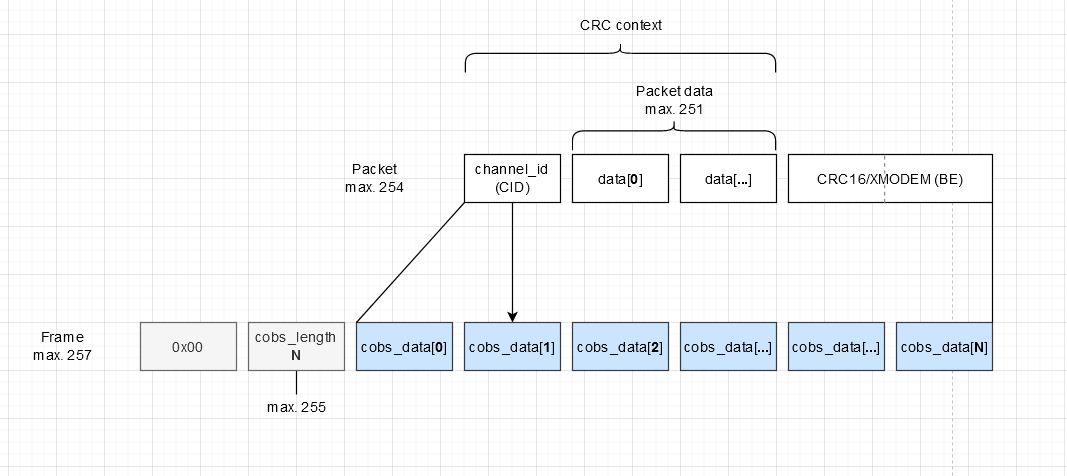
\includegraphics[width=\textwidth]{cobs-diagram}
    \caption{COBS protocol packet structure}
    \label{fig:cobs-diagram}
\end{figure}

The delimiter byte at the start of the packet allows for resetting the packetization state in case a packet is lost, malformed, or other corrupted data is received.


\section{Usage}

((TODO: is this even necessary?))

  - defining a Stream
  - configuring Mux
  - configuring Router
  - creating Consumer


\chapter{Jaculus-device-core}

The Jaculus-device-core library provides a mechanism for defining a Jaculus device and controlling it.

It uses the Jaculus-machine library for the JavaScript runtime and the Jaculus-link library for communication.

% \section{Features}

%   - Jaculus-machine runtime
%   - communication via Jaculus-link
%   - control protocol for controlling and monitoring Jaculus-machine runtime
%   - uploader protocol for uploading code/data to Jaculus device

\section{Architecture}

\subsection{Device class}

The `jac::Device` class is the entry point for defining a Jaculus device. It is a template parametrized by the *Machine* type used for the JavaScript runtime. The *Machine* type must implement the `evalFile` method, which is used to run the code uploaded to the device.

The `jac::Device` class exposes a `jac::Router` object, which is used to connect the device to the communication channel/s. `jac::Device` also exposes an interface for controlling the internal *Machine* instance from C++ code.

Two services are also part of the `jac::Device` class and expose functionality over the communication channel/s:

  - Uploader - service for uploading code/data to the device
  - Controller - service for controlling and monitoring the device

Each service uses a single channel provided by the `jac::Router` object. Other channels are also reserved for the standard input and output of the *Machine* instance and for a global logger instance.

The `jac::Device` implements a locking mechanism to prevent multiple clients from accessing the device simultaneously. The lock is paired with a timeout, which is reset while the client communicates with the devices. If the timeout expires, the lock is released, and other clients can access the device. The lock is exposed to the client via the Controller service.


\section{Implementation}

\subsection{Controller service}

The Controller service is implemented in the `jac::Controller` class. It uses a *PacketCommunicator* interface to communicate with the client. The first byte of each packet is used to specify the command to be executed. The rest of the packet is used to transmit command-specific data.

The service provides the following functionality:

  - accessing the device lock
  - controlling the internal *Machine* instance
  - using the *Machine* instance's standard input and output
  - monitoring the device status

\subsection{Filesystem access}

The Uploader service provides access to the filesystem of the device. Unfortunately, because `std::filesystem` is not yet fully implemented in ESP-IDF, the implementation has to, in some cases, rely on the POSIX filesystem API to be portable to the ESP platform.

\subsection{Uploader service}

The Uploader service is implemented in the `jac::Uploader` class. Similarly to the Controller service, it uses a *PacketCommunicator* interface to communicate with the client. The first byte of each packet is used to specify the command to be executed. The rest of the packet is used to transmit command-specific data.

The service provides the following functionality:

  - listing files and directories
  - creating and deleting directories
  - writing, reading, and deleting files

Most commands are processed in a single packet, but writing files requires the data to be sent in multiple packets. When writing a file, an internal state is set to specify what operation should be performed when data is received and when the transmission is finished. To prevent overflow of the receiving buffer, the command implements, admittedly relatively inefficient, flow control -- the client must acknowledge each packet before the next one is sent.

Commands for reading a file and listing a directory might also split the data into multiple packets. For simplicity, no flow control is implemented when transmitting data to the client, as the client is expected to be a much more powerful device that can handle the transmission.


\section{Usage}

  - defining a Jaculus device
  - controlling a Jaculus device


\chapter{Jaculus-tools}

Jaculus-tools is primarily a command-line application for interacting with Jaculus devices. The application allows users to control and monitor the JavaScript runtime and access the internal filesystem of the device.

It could also be used as a library for building custom applications, but it is not documented. The user might want to look at the source code of the command-line application part of the package for inspiration.

The package is implemented in TypeScript and requires Node.js 18 to run. It can be installed using npm:

```
$ npm install -g jaculus-tools
```


\section{Features}

The application provides the following commands:

  - `help` -- prints help for the specified command
  - `list-ports` -- lists available serial ports
  - `serial-socket` -- tunnels a serial port over a TCP socket
  - `install` -- installs the Jaculus device firmware
  - `build` -- builds the TypeScript code
  - `ls`
  - `read`
  - `write`
  - `rm`
  - `mkdir`
  - `rmdir`
  - `upload`
  - `flash`
  - `pull`
  - `start` -- runs specified file in the device
  - `stop` -- stops the currently running file
  - `status` -- prints the status of the device
  - `monitor` -- connects to the device's standard input and output

The commands are run by specifying them after the `jac` command.

```
$ jac <command> [options] [arguments]
```

\section{Implementation}

\subsection{Command-line argument parser}

The application uses a custom parser for command-line arguments, which allows for chaining compatible commands.

The commands can also access and modify a global state object passed to each command. This allows for commands to share data.

For example, the following command:

```
$ jac --port /dev/ttyUSB0 build flash monitor
```

Will run the three specified commands -- build, flash, monitor -- in sequence. The `build` command compiles the code and saves the compiled code to `build` directory. The `flash` command connects to the device, saves the device to the parser state, and uploads the code. The `monitor` command uses the saved device to access its standard input and output without reconnecting.

Command-line options are divided into two types -- global and command-specific. Options can be specified in any place of the command, as the parsing is done in multiple passes for each specified command. The global options are parsed first, then options of the first command are extracted, then of the second, and so on. Each command then receives only its and the global options. This forces the commands to use different names for their options, as otherwise, preceding commands might extract them. For example, the following two commands would be parsed the same way:

```
$ jac --port /dev/ttyUSB0 build flash monitor
$ jac build flash monitor --port /dev/ttyUSB0
```

The commands can also specify standard arguments, which are parsed after the options:

```
$ jac --port /dev/ttyUSB0 read ./code/index.js
```

\subsection{Connection to the device}

The application implements a simplified version of the interface described in ((TODO - Jaculus-link)) -- the `Router` class is omitted, as connection to multiple devices is pointless. Aside from that and language choice (TypeScript), the implementation is almost identical.

\subsection{Device access}

The application provides access to the device via the `Device` class. The class exposes the following functionality to the user:

  - device lock
  - Controller and Uploader services
  - standard input and output of the running program
  - output of the device logger

\subsection{TypeScript code compilation}



\chapter{Jaculus-esp32}

Jaculus-esp32 is a Jaculus device firmware for the ESP32 family of microcontrollers. It is implemented using the ESP-IDF framework and the Jaculus-device-core library.

\section{Features}

Aside from the features provided by Jaculus-device-core, Jaculus-esp32 only provides control over the most basic peripherals, which are:

  - GPIO -- general-purpose input/output pins
  - ADC -- analog-to-digital converter
  - LEDC -- generator of PWM signals
  - Neopixel -- WS2812B smart LED strip

Jaculus-esp32 also implements a specialized event queue based directly on FreeRTOS queues, supporting scheduling events from an interrupt context. This is used in the GPIO feature for generating events on the input signal change.


\section{Usage}

  - flash manually using ESP-IDF
  - flash using Jaculus-tools


\chapter{Pitfalls}

\section{Only one Context per Machine instance}

From the beginning, the design of Jaculus-machine was to have only one Context per machine. It seemed not to be a limiting factor and simplified implementation. Now it starts to show it was a wrong decision and proves to be a limiting factor in some cases.

For example, in REPL, all exceptions should be caught and reported to standard output. When starting REPL from a JavaScript program, the main program should crash on unhandled exceptions, whereas the REPL should not. Implementation of this would require REPL and the main program to be executed in separate contexts to distinguish between their behavior regarding exception handling.


\section{Unhandled promise rejections not being reported}

This is a limitation of QuickJS. Although QuickJS does have a mechanism for reporting unhandled promise rejections, it reports some false positives. Consider the following example:

``` js
new Promise((resolve, reject) => {
    console.log("promise");
    reject(null);
}).then(() => {
    console.log("ok");
}).catch(() => {
    console.log("error");
});

console.log("after");
```

The promise is created and immediately rejected. At that moment, the promise does not have a rejection handler, and thus QuickJS reports an unhandled promise rejection. However, the handler is added before the promise goes out of scope and handles the rejection.

Fortunately, this is not a problem for well-written code, which handles all possible promise rejections. However, when an unhandled promise rejection occurs, it is not reported, which may lead to errors that are difficult to debug.

To fix this, modifying QuickJS internals would be required, which is outside the scope of this work, but it is an essential consideration for future work.


\section{ESP32 filesystem}

As the filesystem *Feature* is implemented using C++ `std::filesystem`, which is not yet fully supported by the ESP-IDF, some of its functionality might not work, and some may even block the runtime.

The broken functionality involves listing directories -- `readdir` and `rmdir`. Fortunately, working with files works without a problem, which is an essential functionality.


\section{Compatibility with other platforms}

Through implementing all of the created libraries, I have focused on only using the standard C++ library. This worked well for development, as all of the functionality could be tested locally on a desktop PC, and later everything could be easily integrated with the ESP-IDF. Unfortunately, after briefly exploring development options of platforms other than ESP32 (e.g., STM32, RP2040), I have discovered that the C++ 20 standard is not well supported.

This has dealt a significant blow to the portability of the created libraries, which will have to be partially rewritten to support other platforms. Primarily, an abstraction layer around the filesystem and asynchronous elements (e.g., threads, synchronization primitives) will have to be implemented.


\chapter{Comparison with existing solutions}

  - Minimum C/C++ (e.g., ESP-IDF)
  - Arduino (C/C++)
  - NodeMCU (Lua)
  - CircuitPython (Python)
  - Espruino (Javascript)

  - performance
  - memory usage
  - extensibility
  - usability
  - features
  % - no debugger - QuickJS does not support debugging


\chapter{Future work}

  - Web IDE
  - REPL
  - debugger?
  - add more features
  - support more platforms (e.g. STM32, RPi)
  - uploader protocol optimization and stability improvements

\shorthandon{'}
\end{markdown*}
\end{document}
